%!TEX root=main.tex
\section{引言}
\label{socksdirect:sec:intro}

本章的主题是操作系统通信原语加速,在全文中的位置如图 \ref{socksdirect:fig:sys-arch} 所示。

\begin{figure}[htbp]
	\centering
	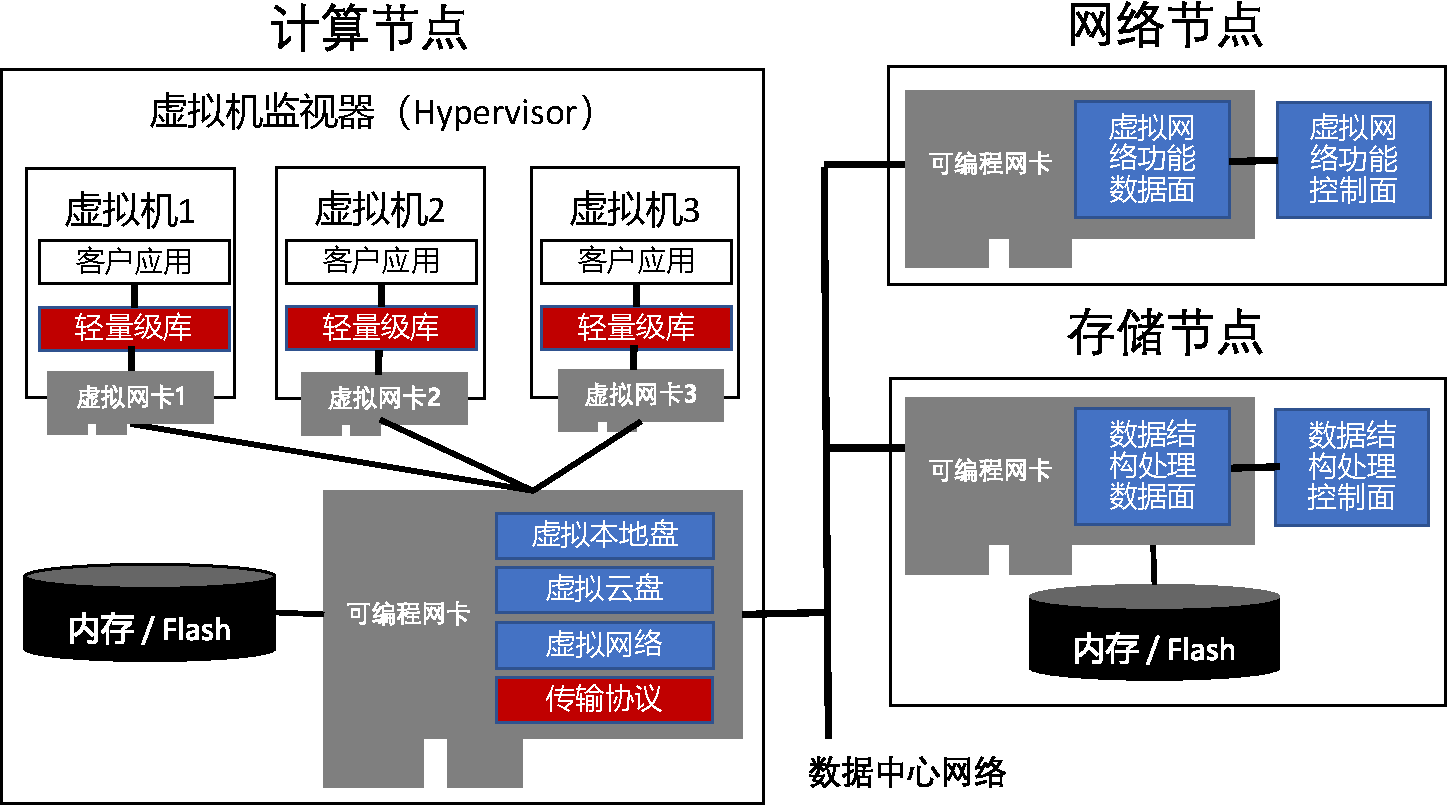
\includegraphics[width=0.8\textwidth]{images/sys_arch.pdf}
	\caption{本章主题:操作系统通信原语加速,用粗斜线背景的方框标出。}
	\label{socksdirect:fig:sys-arch}
\end{figure}

作为本文介绍的最后一个研究工作,本文实现了一个与现有应用兼容的用户态套接字通信库,分别使用共享内存和 RDMA 作为单机进程间和不同主机之间的通信方式。作为补充,基于前面章节提出的 ClickNP 编程框架和 KV-Direct 数据结构处理服务,在可编程网卡内实现了连接数可扩放的 RDMA。

\begin{figure}[htbp]
	\centering
	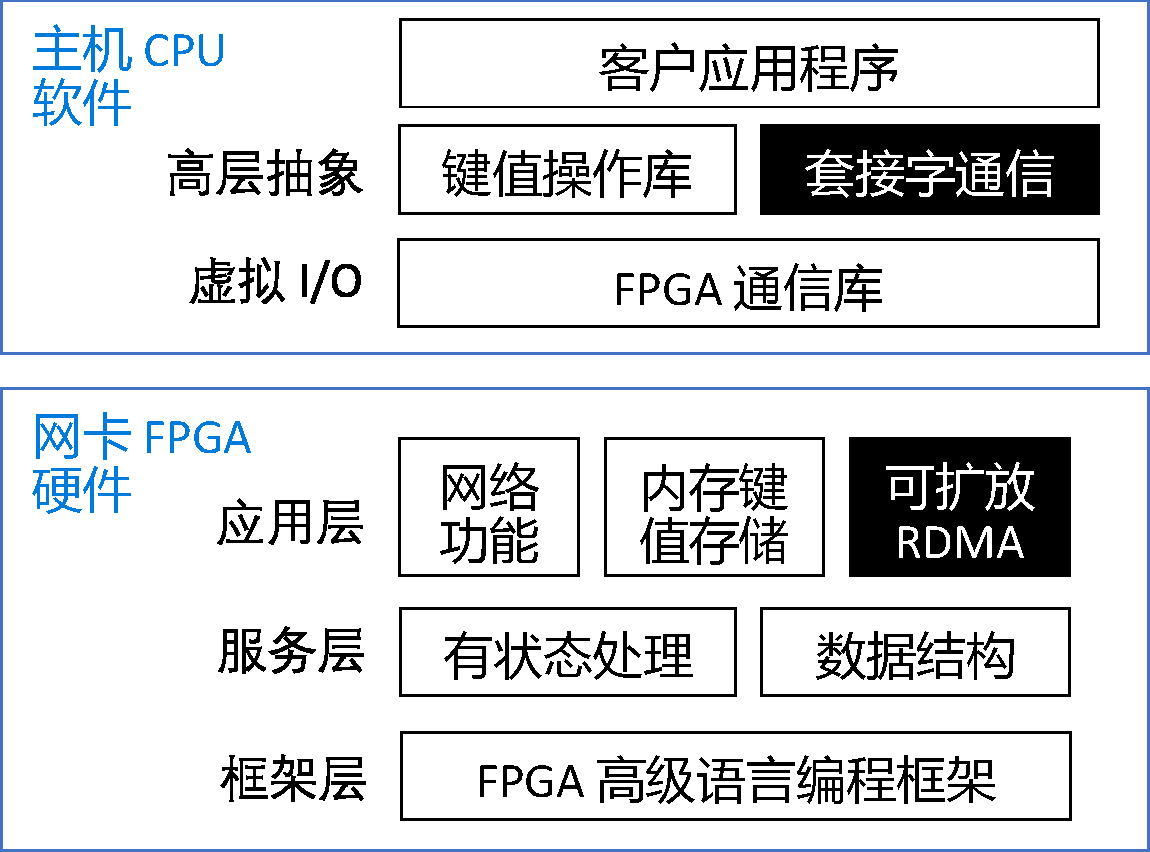
\includegraphics[width=0.5\textwidth]{images/sw_hw_codesign.pdf}
	\caption{本章在可编程网卡软硬件架构中的位置。}
	\label{socksdirect:fig:sw-hw-codesign}
\end{figure}

%Most cloud applications use the socket API for inter-process communication among components or containers inside a same server and across data center network, in addition to serving Internet users. For example, communication intensive applications (\textit{e.g.} Nginx and memcached) spend 50\%$\sim$90\% of CPU time in the OS kernel, mostly processing socket operations.
%The overhead of Linux socket attributes to kernel crossing in system calls, context switch, process scheduling, synchronization, memory copy, cache miss and TCP transport.
%Applications in high performance computing have a long tradition of using shared memory for intra-server communication and RDMA for inter-server, thus avoiding the overheads above.
%However, these abstractions are radically different from socket, so it is complicated and potentially insecure to port socket applications to shared memory and RDMA.
%The overhead of Linux socket becomes salient given the rapid growth of network speed and number of CPU cores per server. %We benchmark communication intensive applications (\textit{e.g.} Nginx and memcached) and find that 50\%$\sim$90\% of CPU time is spent in the OS kernel. When more CPU cores are utilized, they even spend a larger portion of time in the kernel~\cite{boyd2010analysis}. In addition to CPU overhead, latency is also a problem. The round-trip time (RTT) between two processes communicating with shared memory can be as low as 0.2$\mu$s, while TCP socket RTT between two cores is $\approx$16$\mu$s. In a data center, the RTT between RDMA servers is also one order of magnitude lower than kernel TCP/IP stack.

Socket API是现代应用程序中使用最广泛的通信原语,通常用于进程,容器和主机之间的通信。
Linux套接字只能实现比裸的硬件(如共享内存和 RDMA)差一到两个数量级的延迟和吞吐量。
%Socket operations have latency and throughput one order of magnitude worse than the raw hardware.
%Socket operations are expensive and scale poorly with modern multi-core CPUs.
%Communication intensive applications such as distributed key-value stores and web servers could spend 50\%$\sim$90\% of CPU time in the OS kernel~\cite{jeong2014mtcp}, mostly processing socket operations.
近年来,大量工作旨在改善套接字性能。
现有方法或者优化内核网络协议栈 \cite {lin2016scalable,han2012megapipe,yasukata2016stackmap},或者将TCP/IP协议栈移动到用户空间 \cite {jeong2014mtcp,marinos2014network,seastar,fstack,libvma},或者把传输层卸载到RDMA网卡 \cite{rsockets,socketsdirect}。
但是,所有这些解决方案都在兼容性和性能方面存在限制。
它们中的大多数在诸如进程 fork、事件轮询、多应用程序套接字共享和主机内通信等方面与 Linux 套接字不完全兼容。
其中一些 \cite {jeong2014mtcp} 存在隔离问题,不允许多个应用程序共享网卡。
尽管这些工作致力于提升性能,仍有很大的性能提升空间。现有的工作都不能达到接近裸RDMA 和共享内存的性能,因为它们无法消除多线程同步、缓冲区管理和内存复制等重要的开销。
例如,套接字在进程中的多个线程之间共享,因此,许多系统使用锁来避免竞争条件。

%\textcolor{red}{Wei: This seems not promising because socket to RDMA has many solutions.}
%It is often believed that the legacy socket API contributes most to the overheads, so many high performance socket systems propose alternative APIs that require developers to change application code.
%In addition, when the number of active threads is larger than that of CPU cores, polling and kernel event notification are a dilemma.
%Finally, they cannot take advantage of low latency networking provided by RDMA.
%These approaches still have limitations, either not fully removing some of the important overheads such as context switch and synchronization~\cite{lin2016scalable,han2012megapipe,jeong2014mtcp,baumann2009multikernel}, not fully compatible with Linux socket API, or cannot take advantage of modern networking hardware capabilities such as RDMA~\cite{dunkels2001design,jeong2014mtcp,libvma,openonload}.
%There has been extensive work aiming to release the bare metal performance of multi-core CPU and data center network. For intra-server communication, there are mainly three lines of research. The first category of work use the 网卡 as a switch~\cite{peter2016arrakis,belay2017ix,yasukata2016stackmap}, but going deep to the 网卡 introduces $\approx2 \mu$s delay due to PCIe latency, one order of magnitude higher than shared memory. A second line of work optimize or redesign the kernel socket stack~\cite{lin2016scalable,han2012megapipe,jeong2014mtcp,baumann2009multikernel}, where the kernel uses peer-to-peer shared memory communication among cores. However, this approach does not eliminate context switch overhead, while system call batching introduces extra latency. Some other works use dedicated cores as a virtual switch~\cite{huang2017high}, which limits multi-core scalability.

%For inter-server communication, most works leverage a user-space stack~\cite{dunkels2001design,jeong2014mtcp,libvma,openonload} to achieve kernel bypass, but the CPU still needs to handle reliable transport. As RDMA becomes widely available in data centers, we hope to offload the transport to RDMA 网卡s when the peer supports RDMA. Furthermore, most works assume only one connection per pair of processes. However, load balancers, web servers and application gateways serve many concurrent connections~\cite{nishtala2013scaling,lin2016scalable,belay2017ix}. In light of this, both connection setup, event notification and data transmission under high concurrency need to be efficient.

%To demonstrate high performance, most existing works propose new abstractions for inter-process and inter-server communication.  existing socket applications need modifications to use the new abstractions. Furthermore, these stacks are not optimized for a large number of concurrent or short-lived connections, which is an important workload to serve Internet users and large distributed systems.

%One line of research optimize the kernel code or design user-space compatible stacks for higher socket performance. The kernel optimization approach does not eliminate context switch overhead, while system call batching introduces extra latency. User-space stacks are mostly designed for inter-server connections. With the trend of containerized micro-services, we expect an increasing number of applications or containers to be hosted on each server, where inter-process communication (IPC) inside server has more significance.

%To simplify deployment, we hope to accelerate existing applications without modification to the code. \textit{Socket compatibility} adds another dimension of challenge. The socket interface was designed for networking and IPC in millisecond scale, when memory copy, context switch, synchronization, cache miss and cache migration were considered inexpensive~\cite{barroso2017attack,belay2017ix}. An efficient socket architecture for microsecond-scale networking and IPC requires minimizing all overheads above. The semantics lead to challenges. First, the send buffer can be modified by application after non-blocking \texttt{send}, and the receive buffer is not determined until application calls \texttt{recv}. Data copy on \texttt{send} and \texttt{recv} seems mandatory. Second, connections are shared by processes and threads after \texttt{fork} and thread creation. It is challenging to avoid synchronization in this multi-producer and multi-consumer FIFO model. Third, multiple processes listening on a same IP and port compete for incoming connections.

%\textbf{The above part is motivation and related work.}

%The goal of this work is to answer the question: Can a Linux compatible and general purpose socket system provide performance comparable to RDMA systems?

认识到这些限制,本章设计了\sys {},一个用户空间套接字系统,可以同时实现兼容性、隔离性和高性能。
\begin{ecompact}
\item \textbf {兼容性}。
应用程序无需修改,即可使用\sys {} 作为 Linux 套接字的替代品。
\sys{} 同时支持主机内和主机间通信,并且在进程fork和线程创建期间行为正确。
如果远程对端不支持\sys {},则系统将透明地回退到标准TCP。
\item \textbf {隔离性}。
首先,\sys{} 保持了应用程序和容器间的隔离性,即任何应用程序都不能监听或干扰其他应用程序之间的连接,并且一个恶意程序不能使它的连接对端出现错误的行为。
其次,\sys{} 可以实施访问控制策略,以阻止未授权的连接。
\item \textbf {高性能}。
\sys {}提供高吞吐量和低延迟,可与原始RDMA和共享内存相媲美,并可通过多个CPU核心实现性能扩放。
\end{ecompact}


为了实现高性能,\sys{}充分利用了现代硬件的能力。 它利用RDMA进行主机间通信,并使用\emph {共享内存}(shared memory)进行主机内通信。 但是,将套接字操作转换为RDMA和共享内存操作并非易事。
简单的解决方案可能会违反兼容性或在表格上留下很多性能。
例如,在套接字 \textbf {send()}返回后,应用程序可能会覆盖缓冲区。
然而,RDMA 发送操作需要写保护缓冲区。
现有的工作 \cite {rsockets} 或者提供与未修改应用程序不兼容的零拷贝 API,或者需要协议栈管理内部缓冲区并从缓冲区复制数据。
%For example, \textcolor{red}{Take socket send() to RDMA send operations as an example here. If no memory copy, compatibility. If memory copy, performance degradation. Btw, how to point out isolation problem here?}

为了同时实现所有这三个目标,首先需要了解Linux套接字如何提供兼容性和隔离性。 Linux套接字为应用程序提供虚拟文件系统(VFS)抽象。 通过这种抽象,应用程序开发人员可以像操作文件那样进行通信,而无需深入研究网络协议细节。 这种抽象还在共享地址和端口空间的应用程序之间提供了良好的隔离。 但是,VFS抽象非常复杂,许多API本身就不具备可扩展性 \cite {clark1989analysis,boyd2010analysis,jeong2014mtcp}。

尽管VFS具有普遍性和复杂性,许多常用的套接字操作实际上都很简单。因此,本章的设计原则是针对常见情况进行优化,同时保持兼容性。

为了在连接管理中保持隔离的同时加速数据传输,\sys {}将控制和数据平面分开 \cite {peter2016arrakis}。
在每个主机中,引入一个 \emph {管程}(monitor)守护进程作为 \emph {控制平面} 来强制执行访问控制策略,管理地址、端口资源,分派新连接以及在通信对端之间建立传输通道。
\emph {数据平面} 由动态加载的用户空间库\libipc {}处理,它拦截对Linux 标准 C 库的函数调用。 \libipc {}在用户空间中实现套接字API,并将非套接字相关的API转发给内核。
应用程序可以通过在Linux中使用\emph {LD\_PRELOAD}环境变量来加载库来利用\libipc {}。


在\sys {}中,数据传输和事件轮询在对端进程之间直接处理,而连接建立则委托给管程。
本章利用多种技术高效利用硬件并提高系统效率。
通常,线程和fork产生的进程之间共享套接字连接。
为了避免访问套接字元数据和缓冲区带来的竞争条件(race condition),需要同步。
通过基于令牌的共享方法,而不是为每个操作加锁,\sys{} 消除了常见情况下的同步开销。
从网卡发送和接收数据时,现有系统为每个数据包分配缓冲区。
为了消除缓冲区管理开销,本章设计了每个连接独享的环形缓冲区,在发送方和接收方各有一个拷贝,然后利用RDMA和共享内存从发送方环形缓冲区同步到接收方。
为了实现较大消息的零拷贝,\sys{} 利用虚拟内存机制重新映射页面。
%Finally, we observe that cooperative context switch is faster than process wakeup, so we design a mechanism to allow CPU time sharing among polling processes.

\iffalse

We face many challenges designing \sys{}. 
(1) How to share a socket among threads and forked processes without locking?
(2) How to scale to many concurrent connections?
(3) How to utilize shared memory and RDMA efficiently for intra- and inter-host communication?

In both multi-thread and multi-process scenarios, a connection may be shared by multiple senders and receivers.
Existing approaches need locking to protect shared queue and metadata.
To avoid locking overhead, we treat each thread as a separate process.
%, even if the threads have shared memory address space.
\libipc{} uses thread-specific storage and creates peer-to-peer queues between each pair of communicating threads.
To preserve FIFO semantics, we optimize for the common case while prepare for the worst case, and take special care on fork and thread creation.

To handle many concurrent connections efficiently, we need to save memory footprint and improve spatial locality.
For each pair of threads, \sys multiplexes socket connections through one message queue.
Rather than maintaining a separate buffer for each connection and an event notification queue, we receive events and data from the message queue directly.
Observing the event-driven behavior of applications, in normal case the data in queue is fetched by the application in send order.
We design carefully to enable fetching from the middle of queue and solve the head-of-line blocking problem.

We leverage different transports to push performance to the limits of underlying hardware.
For inter-process and inter-container sockets within a same host, we use shared memory in user space.
For sockets among hosts in an RDMA enabled data center, \sys can transparently determine whether the remote endpoint supports \sys.
we fall back to kernel TCP socket.
We design different queue structures for shared memory and RDMA.
We use batched one-sided RDMA write and amortize polling overhead with shared CQ.
%In \sys, sending a small message involves only one cache migration or one-sided RDMA write.
To remove memory copy for large messages, we use \emph{page remapping} to achieve transparent zero copy.
To share a CPU core efficiently among multiple active threads, \sys uses \emph{cooperative multitasking} to remove thread wakeup overhead.

\fi

%The POSIX socket API was designed for networking and IPC in millisecond scale, leading to two performance challenges. First, connections are shared by processes and threads after \texttt{fork} and thread creation. Linux protects this multi-producer multi-consumer FIFO with locks. To scale a shared socket, we \textit{optimize for the common case and prepare for the worst case}. Senders transmit data via different queues in parallel. To ensure receiver ordering, based on the observation that applications seldom receive concurrently from a shared socket, the sender designates a receiver with exclusive access. We further develop mechanisms to avoid deadlock and starvation, in addition to handling unconsumed buffers during \texttt{fork} and thread creation.

%Second, the send buffer can be modified by application after \texttt{send}, and the receive buffer is not determined until application calls \texttt{recv}. Data copy on \texttt{send} and \texttt{recv} seems mandatory. To avoid memory copy of large buffers, we extend the \textit{page remapping} approach~\cite{thadani1995efficient,chu1996zero}, which enables copy-on-write upon \texttt{send} and remaps send buffer to receiver's virtual address upon \texttt{recv}.
%First, we intercept \texttt{memcpy} of full pages to reduce copy-on-write. Second, we move kernel-based page allocation to user-space while preserving security.
%As a result, we achieve zero copy for both shared memory, RDMA and TCP transport.

\sys {}实现了与底层共享内存队列和裸RDMA的性能接近的延迟和吞吐量。
在延迟方面,\sys {} 对主机内套接字实现了0.3微秒RTT,是 Linux的1/35,仅比裸机共享内存队列高出0.05微秒。对于主机间套接字,\sys {} 在RDMA主机之间实现了1.7微秒的RTT,几乎与裸的RDMA写入相同,达到了Linux的1/17。
在吞吐量方面,单个线程可以每秒发送23~M个主机内消息(Linux的20倍)或18~M个主机间(15倍于Linux,1.4倍于裸的RDMA写入)。
对于大型消息,通过零拷贝,单个连接即可饱和利用 100 Gbps 网卡的带宽。
上述性能可随内核数量线性扩放。
\sys {} 为实际应用程序提供了显著的加速。
例如,Nginx~ \cite {nginx} 的HTTP请求延迟降低到了 1/5.5,标准 RPC 库的延迟也可以降低 50%。

总之,本章做出了以下贡献:
\begin{ecompact}
\item 分析Linux套接字的开销。
\item 设计和实现了 \sys {},一个与Linux兼容、能保持应用程序间隔离的高性能用户空间套接字系统。
\item 支持fork、无锁连接共享、环形缓冲区和零拷贝等技术,可能在套接字以外的许多场景中都很有用。
\item 评估显示\sys {}可以实现与RDMA和共享内存队列相当的性能。
\end{ecompact}

%We evaluate end-to-end performance of \sys{} using two categories of applications: \textit{network functions} and \textit{web services}. For a multi-core pipelined network function (NF) chain, a socket application achieves comparable performance with a state-of-the-art NF framework~\cite{panda2016netbricks}. We also evaluate \sys{} on a standard web application composed of a load balancer, a web service and a key-value store.
%For an HTTP request that involves multi-round-trip key-value store accesses, \sys{} reduces end-to-end latency by 2/3.

\iffalse
This paper makes the following contributions:
\begin{ecompact}
	\item A Linux compatible, secure and high performance user-space socket system that supports both inter-process, inter-container and inter-host communication.
	\item A per-host monitor daemon for trusted control plane and peer-to-peer queues for scalable data plane.
	\item A multi-sender and multi-receiver lockless queue to fully support fork and multi-thread socket sharing.
	\item A memory efficient message queue that multiplexes multiple sockets and allows fetching from any socket, while using shared memory and RDMA transports efficiently.
\end{ecompact}
\fi
